\newpage
\section{Implementazione}
In questa sezione vengono analizzati gli aspetti implementativi del sistema, facendo eventualmente riferimento al codice
sviluppato. Nello specifico, verranno approfonditi solamente gli elementi che non sono stati esplorati a pieno nella
sezione Design di Dettaglio o che si ritengono fondamentali nello sviluppo di un progetto di tipo "game" come quello in
discussione.


\subsection{Marcantoni}
Il mio compito all'interno del progetto è stato quello di realizzare il \texttt{GameLoop}, i palloncini (l'entità base,
i vari "potenziamenti" e infine il rispettivo attore), la gestione dei round (con relativa DSL per la loro creazione e
l'attore che si occupa dello \textit{spawn} dei palloncini) e la suddivisione della logica del model nei tre
\textit{manager}. Ho inoltre collaborato con gli altri membri del team durante la fase di design delle entità.

\subsubsection{Game Loop}
Il \textit{game loop} è il ciclo infinito che si occupa di aggiornare il \texttt{Model} ed ordinare il conseguente
\textit{refresh} della \texttt{View}. Solitamente esso viene implementato mediante un ciclo \texttt{while(true)} ma,
avendo adottato il paradigma ad attori, ciò comporterebbe l'esecuzione di un \textit{handler} bloccante con
conseguente perdita totale di reattività da parte dell'attore \texttt{GameLoop}.

Tale effetto è stato evitato mediante un comportamento che sfrutta un \textit{timer}: l'attore \texttt{GameLoop} invia a
se stesso dei messaggi di tipo \texttt{Tick} distanziati tra loro da un \textit{delay} che dipende dal
\textit{frame rate} scelto per la partita. Alla ricezione di tale messaggio il \texttt{GameLoop} ordina al
\texttt{Model} di aggiornarsi; una volta ottenuta la risposta da quest'ultimo, ordina alla \texttt{View} di renderizzare
la lista di entità provenienti dal \texttt{Model}. Le interazioni appena descritte sono riportate in figura
\ref{fig:sequence-gameloop}.

\begin{figure}[H]
  \centering
  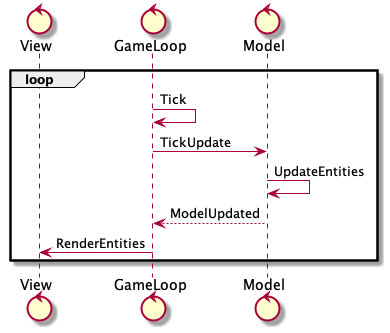
\includegraphics[width=.5\linewidth]{img/sequence-gameloop}
  \caption{Diagramma di sequenza delle interazioni del \texttt{GameLoop}.}
  \label{fig:sequence-gameloop}
\end{figure}

\subsubsection{Palloncini}
I palloncini rappresentano una delle entità fondamentali del gioco. In particolare, essi sono in grado di muoversi
seguendo un percorso e possono essere scoppiati da un proiettile: pertanto, il \texttt{trait Balloon} estende il
\texttt{trait Entity} a cui aggiunge poi le abilità \texttt{TrackFollowing} e \texttt{Poppable} mediante il meccanismo
di \textbf{mixin}.

Per quanto riguarda la loro struttura, i palloncini possono essere \texttt{Simple}, se non ne includono altri al loro
interno, o \texttt{Complex} altrimenti. Tale implementazione permette di rappresentare in modo intuitivo l'effettivo
dominio in quanto, un palloncino complesso, quando scoppiato, deve mostrare il palloncino da lui nascosto.

\begin{lstlisting}[language=Scala, caption=Implementazione dei palloncini, label=lst:balloons]
trait Balloon extends Entity with TrackFollowing with Poppable { ... }
case class Simple(override val ...) extends Balloon
case class Complex(balloon: Balloon) extends Balloon
\end{lstlisting}
Come mostrato nel listato \ref{lst:balloons}, tale implementazione rispecchia quella di un \textbf{sum type}: struttura
dati tipica della programmazione funzionale.

Degni di nota all'interno del \texttt{trait Balloon} sono i metodi \texttt{change} e \texttt{retrieve}. I palloncini
espongono diversi metodi per accedere o cambiare il valore di proprietà che sono contenute all'interno del
\texttt{Simple}. Dato che l'implementazione di tali metodi sarebbe stata pressoché identica, per meglio aderire al
principio DRY si è deciso di introdurre i suddetti due metodi.
Infine, il metodo \texttt{pop} che elimina un numero di \textit{layer} di \texttt{Complex} pari al danno del proiettile
che colpisce il palloncino. Per fare ciò genera, a partire dal palloncino originale, uno \textit{stream} di questi dove
ognuno rappresenta il palloncino risultante dall'esplosione del precedente. L'utilizzo di \texttt{Option} ha permesso,
attraverso il comportamento monadico (sfruttato dal metodo \texttt{flatMap}), di gestire il caso in cui il palloncino
scoppi completamente e di portare avanti la computazione anche in tale situazione.

\begin{lstlisting}[language=Scala, caption=Implementazinoe dei palloncini, label=lst:balloons]
protected[balloons] def retrieve[T](f: Balloon => T): T = this match {
  case Complex(balloon) => balloon retrieve f
  case s => f(s)
}
protected[balloons] def change(f: => Balloon): Balloon = this match {
  case Complex(balloon) => complex(balloon change f)
  case _ => f
}
override def pop(bullet: Bullet): Option[Balloon] = LazyList
  .iterate(Option(this))(_ flatMap {
    case Complex(balloon) => Some(balloon following this)
    case _ => None
  })
  .take(bullet.damage.toInt + 1)
  .last
\end{lstlisting}

